XCTest.frameworkではUIテストを行うことができるが,UIに関するライブラリで利用されていることはまずない.

\href{https://github.com/Instagram/IGListKit}{Instagram/IGListKit: A data-driven UICollectionView framework for building fast and flexible lists.}はデータ駆動のUICollectionViewフレームワークである.プログラム\ref{lstlisting:Instagram/IGListKit:d9a89c9:Tests/IGListAdapterE2ETests.m:137-151}はIGListKit中のテストの1つである.ここでは,{\sf setUp}メソッドと{\sf setupWithObjects}メソッドでテスト環境を用意し,{\sf waitForExpectationsWithTimeout}で待機する間に{\sf UICollectionView}に対するアサーションを行っている.

\begin{lstlisting}[language=objectivec,caption=\href{https://github.com/Instagram/IGListKit/blob/d9a89c9b00aa1a9537a24d9affb6919f83065f65/Tests/IGListAdapterE2ETests.m}{UIライブラリにおけるアサーションを用いたテスト},label=lstlisting:Instagram/IGListKit:d9a89c9:Tests/IGListAdapterE2ETests.m:137-151,firstnumber=137]
- (void)test_whenUpdatesComplete_thatCellsExist {
    [self setupWithObjects:@[
                             genTestObject(@1, @2),
                             genTestObject(@2, @2),
                             ]];
    XCTestExpectation *expectation = genExpectation;
    [self.adapter performUpdatesAnimated:YES completion:^(BOOL finished) {
        XCTAssertNotNil([self.collectionView cellForItemAtIndexPath:[NSIndexPath indexPathForItem:0 inSection:0]]);
        XCTAssertNotNil([self.collectionView cellForItemAtIndexPath:[NSIndexPath indexPathForItem:1 inSection:0]]);
        XCTAssertNotNil([self.collectionView cellForItemAtIndexPath:[NSIndexPath indexPathForItem:0 inSection:1]]);
        XCTAssertNotNil([self.collectionView cellForItemAtIndexPath:[NSIndexPath indexPathForItem:1 inSection:1]]);
        [expectation fulfill];
    }];
    [self waitForExpectationsWithTimeout:30 handler:nil];
}
\end{lstlisting}

スクリーンショット(スナップショット)をテストに利用しているライブラリも存在する.iOSアプリケーションでスクリーンショットを撮る方法としては以下の3つがある.

\begin{itemize}
    \item XCTest.frameworkの{\sf XCUIScreenshot}の利用
    \item \href{https://github.com/facebook/ios-snapshot-test-case}{facebook/ios-snapshot-test-case: Snapshot view unit tests for iOS}の利用
    \item \href{https://github.com/fastlane/fastlane/tree/master/snapshot}{fastlane/snapshot at master · fastlane/fastlane}の利用
\end{itemize}

ios-snapshot-test-caseは{\sf UIView}や{\sf CALayer}の画像を取得することによる,アプリケーションテスト用のライブラリである.得られた画像とリポジトリ内の画像が一致しない場合テストは失敗となる.スクリーンショットを用いたテストにより,デザイナーと連携したりテストカバレッジを向上させたりする効果があるとされる\cite{objc.io:snapshot-testing}.

グラフ描画ライブラリ\href{https://github.com/danielgindi/Charts}{danielgindi/Charts: Beautiful charts for iOS/tvOS/OSX! The Apple side of the crossplatform MPAndroidChart.}ではこのライブラリを利用している.プログラム\ref{lstlisting:danielgindi/Charts:d300d6d:Tests/Charts/BarChartTests.swift:50-53}はその一例である.また,図\ref{figure:danielgindi/Charts:d300d6d:Tests/ReferenceImages_64/ChartsTests.BarChartTests/testDefaultValues_iOS_320.0_568.0@2x.png}はプログラム\ref{lstlisting:danielgindi/Charts:d300d6d:Tests/Charts/BarChartTests.swift:50-53}内のスクリーンショットに対応する画像の1つである.{\sf setUp}メソッドで描画するデータを与え,{\sf testDefaultValues}はじめとするテストメソッドで描画結果を確認している.

\begin{lstlisting}[language=swift,caption=\href{https://github.com/danielgindi/Charts/blob/d300d6d332afa2e790fd616e5a8326e815b0e1f0/Tests/Charts/BarChartTests.swift}{UIライブラリにおけるスクリーンショットを用いたテスト},label=lstlisting:danielgindi/Charts:d300d6d:Tests/Charts/BarChartTests.swift:50-53,firstnumber=50]
    func testDefaultValues()
    {
        FBSnapshotVerifyView(chart, identifier: Snapshot.identifier(UIScreen.main.bounds.size), tolerance: Snapshot.tolerance)
    }
\end{lstlisting}

\begin{figure}
    \centering
    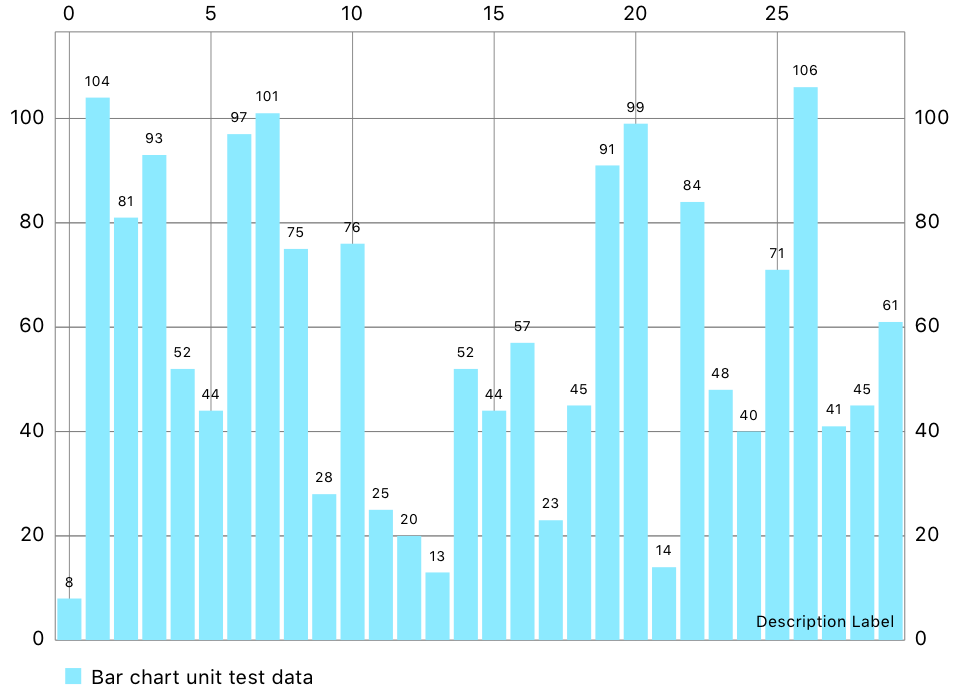
\includegraphics[width=10cm]{images/bodies/thirdparty/case/testDefaultValues.png}
    \caption{スクリーンショットを用いたテストと対応する画像}
    \label{figure:danielgindi/Charts:d300d6d:Tests/ReferenceImages_64/ChartsTests.BarChartTests/testDefaultValues_iOS_320.0_568.0@2x.png}
\end{figure}

ios-snapshot-test-caseを利用しているライブラリとしては次のようなものがある.括弧内は確認したコミット番号である.

\begin{itemize}
    \item \href{https://github.com/facebookarchive/AsyncDisplayKit}{facebookarchive/AsyncDisplayKit: Smooth asynchronous user interfaces for iOS apps.}(5df7456c56e3fd579783b8816aacb82cc6c1abd1)
    \item \href{https://github.com/dzenbot/DZNEmptyDataSet}{dzenbot/DZNEmptyDataSet: A drop-in UITableView/UICollectionView superclass category for showing empty datasets whenever the view has no content to display}(b5b9216d09f19455aa616d3bda32e1c38d3178bd)
    \item \href{https://github.com/danielgindi/Charts}{danielgindi/Charts: Beautiful charts for iOS/tvOS/OSX! The Apple side of the crossplatform MPAndroidChart.}(8245f32498739cde83dc729123d58538184b78f5)
\end{itemize}

ブログに紹介されている33個のライブラリのうちfastlaneを使用しているのは\href{https://github.com/onevcat/Kingfisher}{onevcat/Kingfisher: A lightweight, pure-Swift library for downloading and caching images from the web.}(037c3ec78bb77cb16a6f3076006f718fd66283c6)と\href{https://github.com/onevcat/Hedwig}{onevcat/Hedwig: Send email to any SMTP server like a boss, in Swift and cross-platform}(8e3b629982eb9f2576225400819482164b6e248d)の2個で,どちらもテストやGitHubへのリリースに使用しておりsnapshot機能は使用していない.
